\section{Distributed Systems}

    A distributed system can be defined as a number of autonomous computing elements which 
    appear to a user as a single coherent system. \cite[p.~2]{DistributedSystems}. 
    This definition states that a complex system being split apart into meaningful domains
    each being able to behave independently of each other. These individual elements 
    mentioned could be either a hardware device or possibly a software process. It is also 
    a feature of distributed systems to make the application user believe that a only a system 
    is being used. 

    \begin{figure}[htbp!]
        \centering 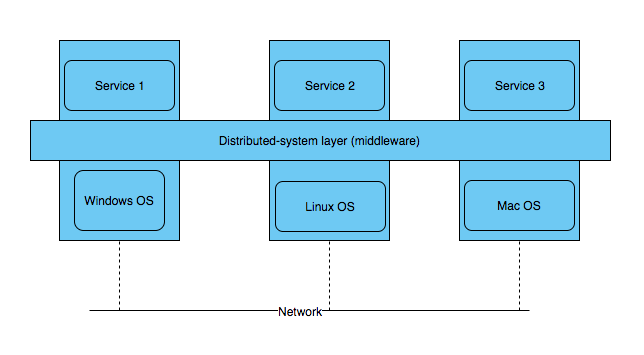
\includegraphics[scale=0.94]{grafiken/distributedSystem.png}
        \caption{A distributed system extended over multiple machine with same application interface \cite{DistributedSystems}}
        \label{fig:distributedSystem}
    \end{figure}

    \newpage
    \par
        Figure \ref{fig:distributedSystem} shows an example of an application being 
        distributed amongst different computers. It can also be seen that the application
        is allowed to communicate via a common middleware whose main responsibility is to
        efficiently manage resources across the distributed applications. This kind of system
        makes most sense for deployment which require high performance computing with fairly
        large number of domains\footnotemark[\value{footnote}].
        \footnotetext {domain: A subject area to which the user applies the program in a 
        software \cite{DDD}.}

    \par
        Distributed systems can be utilized to realize a complex application with smaller
        autonomous independent entities which communicates via a network protocol. The 
        components interacts with each other to achieve a common goal. It also provides
        more reliability than a non-distributed system because there is no single point
        of failure. 
        

        